\begin{flushright}
    \textit{Лекция 19 (от 09.11)}
\end{flushright}
\begin{center}
    \textbf{Функция Жуковского}
\end{center}
\begin{equation}\label{(24.1)}
    w = \frac{1}{2}\left( z+\frac{1}{z} \right)
\end{equation}
Заметим, что $0$ и $\infty$~--- полюсы $1$ порядка, $\pm 1$~--- нули
производной.
\\
В каждой точке $z \not \in \left\{0, \pm 1,\infty \right\}$ функция конформна. В
точке $0$
\begin{align*}
  & g(z) = \frac{1}{w(z)} = \frac{2z}{z^2+1}
\end{align*}
Эта функция в нуле регулярна и имеет ненулевую производную, а значит, конформна
в нуле. В точке $\infty$
\begin{align*}
  & \varphi(z) = w\left( \frac{1}{z} \right) = \frac{1}{2}\left( \frac{1}{z} + z \right)
\end{align*}
Заметим, что это та же $w$, и в силу конформности в нуле конформна и на
бесконечности. В остальных точках проверим однолистность.
\begin{align*}
  & \frac{1}{2}\left( z_1 + \frac{1}{z_1} \right) - \frac{1}{2}\left( z_1 + \frac{1}{z_1} \right) = 0
\end{align*}
\begin{align*}
  & (z_1-z_2) \left( 1-\frac{1}{z_1z_2} \right)
\end{align*}
\begin{align*}
  & \left[ \begin{matrix}
          z_1=z_2 \\
          z_1z_2 = 1
      \end{matrix} \right.
\end{align*}
Область однолистности $G$: $\pm 1 \not \in G$, $\forall z \in G \ \dst
\frac{1}{z} \not \in G$.
\Example
Функция $w = \dst \frac{1}{z}$ задает две симметрии: относительно единичной
окружности и относительно действительной оси. Соответственно, области
однолистности:
\begin{itemize}
    \item $\left| z \right| < 1$
    \item $\left| z \right| > 1$
    \item $\Img z > 0$
    \item $\Img z < 0$
\end{itemize}
Пусть $z = e^{i \varphi}$, тогда функция Жуковского:
\begin{align*}
  & w = \frac{1}{2}\left( e^{i \varphi} + e^{-i\varphi}\right)
\end{align*}
\begin{equation}\label{(24.2)}
    \begin{cases}
        u = \frac{1}{2}\left( r+\frac{1}{r} \right)\cos \varphi \\
        v = \frac{1}{2}\left( r-\frac{1}{r} \right)\sin \varphi
    \end{cases}
\end{equation}
\Example
~
\begin{itemize}
    \item Пусть задана окружность
    \begin{align*}
      \gamma_r = \left\{ z: \left| z \right| = r, \ r \neq 1\right\}
    \end{align*}
    \begin{align*}
      & \frac{u^2}{a^2} + \frac{v^2}{b^2} = 1, \ a = \frac{1}{2}\left( r + \frac{1}{r} \right), \ b = \frac{1}{2}\left|  r - \frac{1}{r} \right|
    \end{align*}
    \begin{align*}
      & a^2+b^2 = c^2 = 1
    \end{align*}
    Такая окружность переходит в эллипс с фокусами в $\pm 1$, действительной
    полуосью $a$ и мнимой $b$.
    \item Пусть задан луч
    \begin{align*}
      l_\varphi = \left\{ z \mid z = re^{i\varphi}, \ r > 0\right\}, \ \varphi \in [-\pi;\pi) \setminus \left\{ 0, \pm \frac{\pi}{2}, -\pi \right\}
    \end{align*}
    \begin{equation}\label{(24.3)}
        \frac{u^2}{\cos^2 \varphi} - \frac{v^2}{\sin^2\varphi} = 1
    \end{equation}
    Такой луч переходит в гиперболу с фокусами в $\pm 1$.
    \begin{itemize}
        \item $\varphi \in \left( 0; \dst \frac{\pi}{2} \right)$~--- отображение
        в правую ветвь гиперболы, движение по ней вверх.
        \item $\varphi \in \left(\dst \frac{\pi}{2}; \pi \right)$~---
        отображение в левую ветвь гиперболы, движение по ней вверх.
        \item $\varphi \in \left( - \dst \frac{\pi}{2}; 0 \right)$~---
        отображение в правую ветвь гиперболы, движение по ней вниз.
        \item $\varphi \in \left( -\pi; -\dst \frac{\pi}{2} \right)$~---
        отображение в левую ветвь гиперболы, движение по ней вниз.
    \end{itemize}
\end{itemize}
\Example
~
\\
\begin{figure}[h!]
    \begin{minipage}[c]{0.45\textwidth}
        \centering
        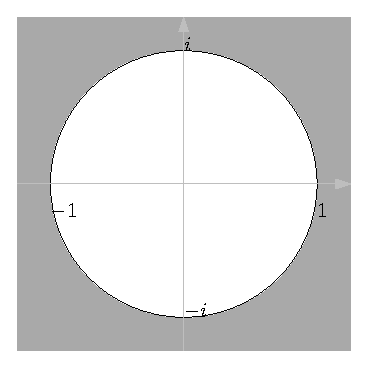
\includegraphics[scale=0.75]{rnd_in.eps}
    \end{minipage}
    \begin{minipage}[c]{0.1\textwidth}
        \centering
        \LARGE{$\mapsto$}
    \end{minipage}
    \begin{minipage}[c]{0.45\textwidth}
        \centering
        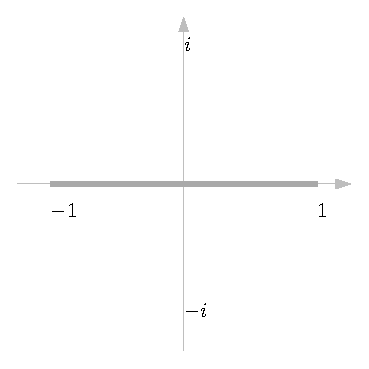
\includegraphics[scale=0.5]{pm1.eps}
    \end{minipage}
    \label{fig:24.10}
    \caption{Перевод единичного круга в $\CC \setminus [-1;1]$}
\end{figure}
\FloatBarrier
\Example
~
\\
\begin{figure}[h!]
    \begin{minipage}[c]{0.45\textwidth}
        \centering
        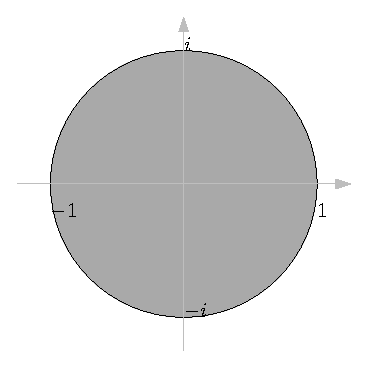
\includegraphics[scale=0.75]{rnd_out.eps}
    \end{minipage}
    \begin{minipage}[c]{0.1\textwidth}
        \centering
        \LARGE{$\mapsto$}
    \end{minipage}
    \begin{minipage}[c]{0.45\textwidth}
        \centering
        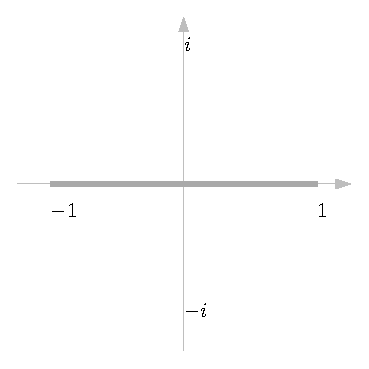
\includegraphics[scale=0.5]{pm1.eps}
    \end{minipage}
    \label{fig:24.11}
    \caption{Перевод внешности единичного круга в $\CC \setminus [-1;1]$}
\end{figure}
\FloatBarrier
\Example
~
\\
\begin{figure}[h!]
    \begin{minipage}[c]{0.45\textwidth}
        \centering
        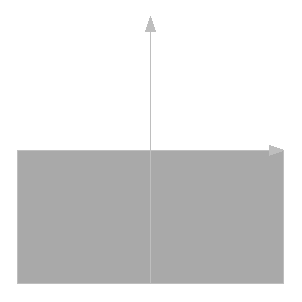
\includegraphics[scale=0.75]{half_plane.eps}
    \end{minipage}
    \begin{minipage}[c]{0.1\textwidth}
        \centering
        \LARGE{$\mapsto$}
    \end{minipage}
    \begin{minipage}[c]{0.45\textwidth}
        \centering
        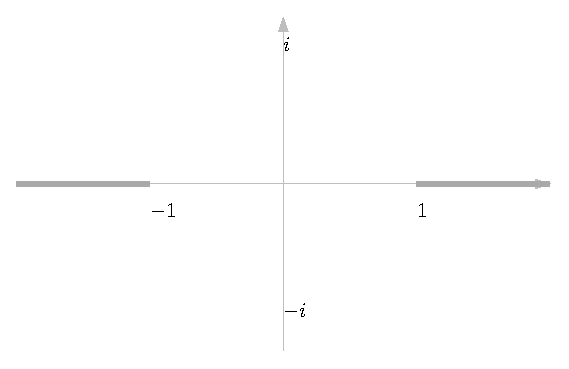
\includegraphics[scale=0.5]{pm1out.eps}
    \end{minipage}
    \label{fig:24.12}
    \caption{Перевод верхней полуплоскости в $\CC \setminus ((-\infty;-1]\cup[1;+\infty)$}
\end{figure}
\FloatBarrier
\Example
~
\\
\begin{figure}[h!]
    \begin{minipage}[c]{0.45\textwidth}
        \centering
        
\includegraphics[scale=0.75]{half_plane_t.eps}
    \end{minipage}
    \begin{minipage}[c]{0.1\textwidth}
        \centering
        \LARGE{$\mapsto$}
    \end{minipage}
    \begin{minipage}[c]{0.45\textwidth}
        \centering
        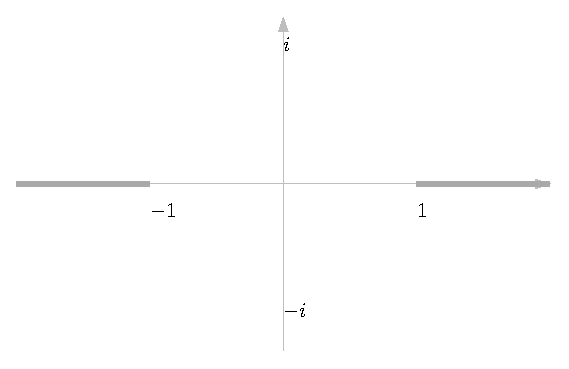
\includegraphics[scale=0.5]{pm1out.eps}
    \end{minipage}
    \label{fig:24.13}
    \caption{Перевод нижней полуплоскости в $\CC \setminus ((-\infty;-1]\cup[1;+\infty)$}
\end{figure}
\FloatBarrier
Отыщем обратную функцию Жуковского.
\begin{align*}
  & w = \frac{1}{2}\left( z+\frac{1}{z} \right) \Rightarrow z^2 - 2wz + 1 = 0
\end{align*}
\begin{align*}
  & z = w \pm g(w), \ g(w) \in \sqrt{w^2-1}
\end{align*}
\Example
Ветвь обратной функции Жуковского, где $g \sim w$ при $w \to \infty$, $z = w -
g(w)$, выполняет следующее преобразование:
\\
\begin{figure}[h!]
    \begin{minipage}[c]{0.45\textwidth}
        \centering
        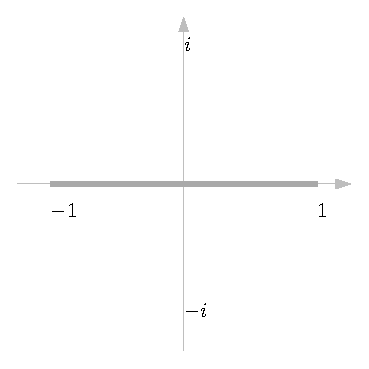
\includegraphics[scale=0.5]{pm1.eps}
    \end{minipage}
    \label{fig:24.14}
    \begin{minipage}[c]{0.1\textwidth}
        \centering
        \LARGE{$\mapsto$}
    \end{minipage}
        \begin{minipage}[c]{0.45\textwidth}
        \centering
        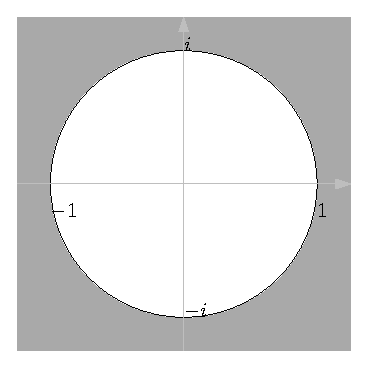
\includegraphics[scale=0.75]{rnd_in.eps}
    \end{minipage}
    \caption{Перевод $\CC \setminus [-1;1]$ в единичный круг}
\end{figure}
\FloatBarrier
\Example
Ветвь обратной функции Жуковского, где $g \sim w$ при $w \to \infty$, $z = w +
g(w)$, выполняет следующее преобразование:
\\
\begin{figure}[h!]
        \begin{minipage}[c]{0.45\textwidth}
        \centering
        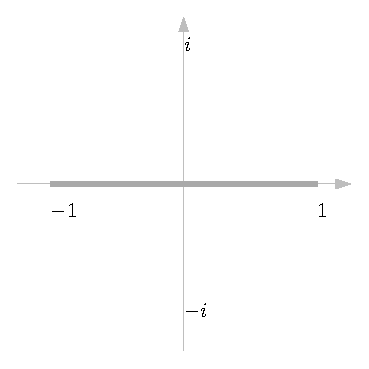
\includegraphics[scale=0.5]{pm1.eps}
    \end{minipage}
    \begin{minipage}[c]{0.1\textwidth}
        \centering
        \LARGE{$\mapsto$}
    \end{minipage}
        \begin{minipage}[c]{0.45\textwidth}
        \centering
        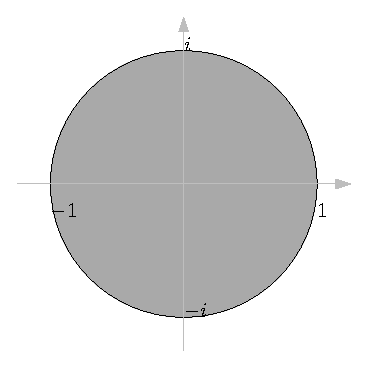
\includegraphics[scale=0.75]{rnd_out.eps}
    \end{minipage}
    \label{fig:24.15}
    \caption{Перевод $\CC \setminus [-1;1]$ во  внешность единичного круга}
\end{figure}
\FloatBarrier
\Example
Ветвь обратной функции Жуковского, где $g(0) = i$, $z = w - g(w)$, выполняет
следующее преобразование:
\\
\begin{figure}[h!]
        \begin{minipage}[c]{0.45\textwidth}
        \centering
        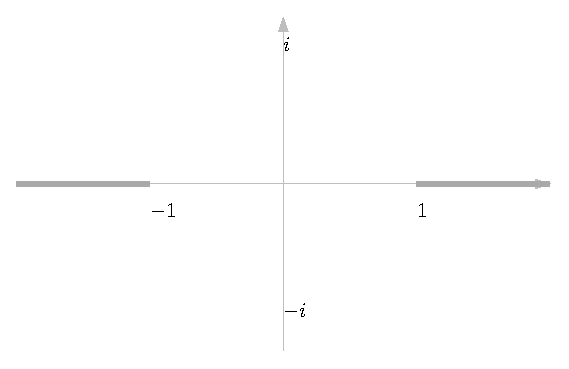
\includegraphics[scale=0.5]{pm1out.eps}
    \end{minipage}
    \begin{minipage}[c]{0.1\textwidth}
        \centering
        \LARGE{$\mapsto$}
    \end{minipage}
    \begin{minipage}[c]{0.45\textwidth}
        \centering
        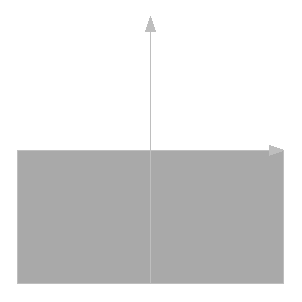
\includegraphics[scale=0.75]{half_plane.eps}
    \end{minipage}
    \label{fig:24.16}
    \caption{Перевод $\CC \setminus (-\infty;-1]\cup[1;+\infty)$ в верхнюю полуплоскость}
\end{figure}
\FloatBarrier
\Example
Ветвь обратной функции Жуковского, где $g(0) = i$, $z = w + g(w)$, выполняет
следующее преобразование:
\\
\begin{figure}[h!]
        \begin{minipage}[c]{0.45\textwidth}
        \centering
        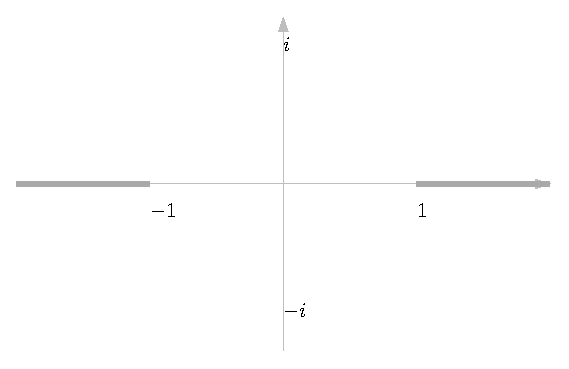
\includegraphics[scale=0.5]{pm1out.eps}
    \end{minipage}
    \begin{minipage}[c]{0.1\textwidth}
        \centering
        \LARGE{$\mapsto$}
    \end{minipage}
    \begin{minipage}[c]{0.45\textwidth}
        \centering
        
\includegraphics[scale=0.75]{half_plane_t.eps}
    \end{minipage}
    \label{fig:24.17}
    \caption{Перевод $\CC \setminus (-\infty;-1]\cup[1;+\infty)$ в нижнюю полуплоскость}
\end{figure}
\FloatBarrier
\begin{center}
    \textbf{Теорема Римана}
\end{center}
$\CC$ нельзя конформно отобразить на единичный круг. Действительно, функция (в
предположении существования) будет ограничена, регулярна (в силу определенности
на всей комплексной плоскости она обязана быть целой), значит, по теореме
Лиувилля это константа, что не является требуемым отображением.
\theorem
Общий вид конформного отображения $B_1(0) \mapsto B_1(0)$:
\begin{equation}\label{(24.4)}
    f(z) = e^{i\beta}\frac{z-a}{1-z\ol{a}}
\end{equation}
\pr
Если $f$ удовлетворяет \eqref{(24.4)}, то $f: B_1(0) \mapsto B_1(0)$ есть ДЛО, а
значит, оно конформно.
\\
Пусть теперь $g: B_1(0) \mapsto B_1(0)$~--- некоторое конформное отображение.
Докажем, что такая функция удовлетворяет \eqref{(24.4)}.
\\
Заметим:
\begin{align*}
  \exists w_0 \in B_1(0): \ g(0) = w_0
\end{align*}
Расмотрим теперь
\begin{align*}
  h(w) = \frac{w-w_0}{1-w\ol{w_0}}, \ h(w_0) = 0, \ h:B_1(0)\mapsto B_1(0)
\end{align*}
Положим
\begin{align*}
  f(z) = h(g(z))
\end{align*}
$f$ регулярна, как суперпозиция регулярных функций, и причем $f(0) = 0$,
$f:B_1(0) \mapsto B_1(0)$. Тогда по лемме Шварца $\forall z \in B_1(0) \ \left|
    f(z) \right|\leq \left| z \right|$.
\\
Тогда $f^{-1}$ таже будет регулярна, $f^{-1}(0) = 0$, $f^{-1}: B_1(0) \mapsto
B_1(0)$. Тогда по лемме Шварца $\forall w \in B_1(0) \ \left| f^{-1}(w)
\right|\leq \left| w \right|$. Подставляя сюда $w = f(z)$, получим $\left| z
\right| \leq \left| f(z) \right|$, т.~е. $\left| z \right| = \left| f(z)
\right|$, и по лемме Шварца выполняется $f(z) = e^{i\alpha}z$.
\\
Тогда $g(z)$~--- ДЛО. Проверим, что $g$ имеет вид \eqref{(24.4)}.
\begin{align*}
& e^{i\alpha}z = h^{-1}(g(z)); \ \exists z_0 \in B_1(0): \ g(z_0) = 0
\end{align*}
\begin{align*}
& e^{i\alpha} = (h^{-1})'(0)(g'(z_0)) = \frac{g'(z_0)}{h'(w_0)}
\end{align*}
\begin{align*}
& \alpha \in \Arg g'(z_0) - \Arg h'(w_0)
\end{align*}
\begin{align*}
& h'(w_0) = \left.\frac{1-w\ol{w_0}+\ol{w_0}(w-w_0)}{(1-w\ol{w_0})^2}\right|_{w=w_0} = 1 - \left| w_0 \right|^2 > 0 \Rightarrow 0 \in \Arg h'(w_0)
\end{align*}
\begin{align*}
& \alpha \in \Arg g'(z_0)
\end{align*}
Рассмотрим теперь 
\begin{align*}
& g_1(z) = e^{i\alpha}\frac{z-z_0}{1-z\ol{z_0}}
\end{align*}
\begin{align*}
&\varphi(z) = g(g_1^{-1}(w)): B_1(0) \mapsto B_1(0)
\end{align*}
\begin{align*}
&\varphi(g_1(z)) = g(w), \ \varphi(0) = 0, \ \Arg \varphi'(0) + \Arg g_1'(0) = \Arg g'(z_0)
\end{align*}
Дифференцируя,
\begin{align*}
& \alpha \in \Arg g_1(0), \ 0 \in \Arg \varphi'(0)
\end{align*}
По лемме Шварца для прямой и обратной функций
\begin{align*}
& \left| \varphi(z) \right| = \left| z \right| \Rightarrow \varphi(z) = z
\end{align*}
(в силу $0 \in \Arg \varphi'(0)$). Но тогда $g_1(z) = g(z)$, и теорема
доказана.
\lemma 
Пусть область $G\subseteq \CC$ такова, что существует конформное $f_0: G \mapsto
B_1(0)$. Тогда любое конформное отображение $G$ на $B_1(0)$ имеет вид
\begin{align*}
  & f(z) = h(f_0(z))
\end{align*}
причем $h$ имеет вид \eqref{(24.4)}.
\pr
Пусть $f_1: G \mapsto B_1(0)$~--- конформное. Рассмотрим 
\begin{align*}
  & \varphi(w) = f_1(f_0^{-1}(w)): B_1(0) \mapsto B_1(0)
\end{align*}
Оно конформно как суперпозиция конформных. По теореме $1$ это ДЛО,
уловлетворяющее \eqref{(24.4)}. Поскольку
\begin{align*}
& f_1(z) = \varphi(f_0(z))
\end{align*}
то лемма доказана.
\theorem (единственности конформных отображений)
Пусть $G$ такова, что существует конформное $f_0:G \mapsto B_1(0)$. Тогда
множество всех конформных отображений $G \mapsto B_1(0)$ зависит от трех
действительных параметров. В частности, такое отображение единственно, если
выполнены условия:
\begin{equation}\label{(24.5)}
f(z_0) = 0, \ \argt f'(z_0) = \alpha \in [0;2\pi), \ z_0 \in G
\end{equation}
\pr
Из леммы $1$ и теоремы $1$ следует утверждение о трех параметрах.
\\
Докажем теперь единственность. Допустим, от противного, существуют $f_1$, $f_2$,
удовлетворяющие \eqref{(24.5)}. Пусть
\begin{align*}
  & \varphi(w) = f_1(f_2^{-1}(w)), \ \varphi(f_2(z)) = f_1(z), \ \varphi(0) = 0
\end{align*}
Значит, $\varphi(z)$ будет ДЛО по лемме $1$. Дифференцируя в $z_0$, имеем
\begin{align*}
    & \argt \varphi'(0) + \Arg f_2'(z_0) = \Arg f_1'(z_0)
\end{align*}
\begin{align*}
  & 0 \in \Arg \varphi'(0) \Rightarrow \varphi(0) = 0, \ z_0 = 0, \ \alpha = 0
\end{align*}
\begin{align*}
  & \varphi(z) = z \Rightarrow f_1(z) = f_2(z)
\end{align*}
\theorem (Римана)
Пусть $G$~--- область в $\CCC$, граница которой содержит более одной точки.
Тогда существует конформное $f: G \mapsto B_1(0)$.
\corollary
Если $G_1 \subseteq \CCC$, $G_2 \subseteq \CCC$, и ганицы каждой содержат более
одной точки, то существует конформное обображение $G_1$ на $G_2$.
\pr
Пусть $f_1: G_1 \mapsto B_1(0)$, $f_2: G_2 \mapsto B_1(0)$, тогда искомое
отображение $\varphi(z) = f_1(f_2^{-1}(z)): G_1 \mapsto G_2$.
\theorem (принцип соответствия границ)
Пусть $G_1, G_2$~--- ограниченные односвязные области в $\CC$ с кусочно гладкими
границами $\Gamma_1, \Gamma_2$. Пусть $f: G_1 \mapsto G_2$~--- конформное; тогда
существует непрерывное продолжение $\tilde{f}$ такое, что оно отображает
$\Gamma_1$ на $\Gamma_2$ с сохранением ориентации.